% !TEX program = xelatex

\documentclass{resume}
%\usepackage{zh_CN-Adobefonts_external} % Simplified Chinese Support using external fonts (./fonts/zh_CN-Adobe/)
%\usepackage{zh_CN-Adobefonts_internal} % Simplified Chinese Support using system fonts
\usepackage{zh_CN-Adobefonts_external} % Simplified Chinese Support using external fonts (./fonts/zh_CN-Adobe/)
%\usepackage{NotoSansSC_external}
%\usepackage{NotoSerifCJKsc_external} \usepackage{zh_CN-Adobefonts_internal} % Simplified Chinese Support using system fonts
\usepackage{linespacing_fix} % disable extra space before next section
\usepackage{cite}
\usepackage{graphicx}
\usepackage{tabu}
\usepackage{multirow}
\usepackage{progressbar}
\begin{document}
	
	\pagenumbering{gobble} % suppress displaying page number
	
	\begin{center}
		\Large
		\begin{tabu}{ c l r }
			\multirow{5}{1in}{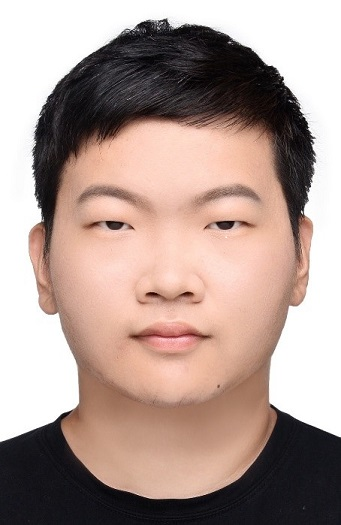
\includegraphics[width=0.12\textwidth]{cd2}} & \scshape{Chang Di} & {Python~}\progressbar{0.9} \\
			& \email{2862588711cd@gmail.com} & {Matlab}\progressbar{0.9} \\
			& \phone{(+86) 188-428-32169} & {Latex}\progressbar{0.8} \\
			& \linkedin[Chang Di]{https://www.linkedin.com/in/chang-di-004784206} & {C}\progressbar{0.6} \\
			& \github[Boese0601]{https://github.com/Boese0601} & {Javascript}\progressbar{0.6}
		\end{tabu}
	\end{center}
	
	
	
	\basicInfo{}
	
	\section{\faGraduationCap\  Education Background}
	\datedsubsection{\textbf{Dalian University of Technology}, Dalian,Liaoning}{2018.9 -- Present}
	\textit{B.Eng}\ Electronic and Information Engineering, Expected to graduate in 2022.9
	\begin{itemize}
		\item Cumulative GPA : 91.1/100 \quad 3.91/4.0 \qquad|| \qquad Major GPA : 93.0/100\quad 3.95/4.0 
		\item Ranking : 10/210   \qquad   Top 5 \%
		\item Selected Outstanding Coureses : Mathematics Analysis:100\quad Computer Organization:96 \\
		 Digital Circuit:96 \quad Discrete Mathematics:98 \quad Probability and Statistics:98 \quad Data Structure:93
	\end{itemize}
	\datedsubsection{\textbf{Technical University of Munich}, Munich, Bayern}{2021.10 -- 2022.9}
	\textit{Exchange Student}\ Informatics,already been admitted,leave for TUM in 2021.10 
	\datedsubsection{\textbf{Imperial College London}, London}{2021.1 -- 2021.3}
	\textit{Winter School}\ Data Science and Computer Vision
	\datedsubsection{\textbf{University of California,San Diego}, San Diego,California}{2019.6 -- 2019.8}
	\textit{Summer Session}\ Electrical and Computer Engineering\\
	Introduction to Deep Learning A+ 4.0/4.0\\
	American culture and history  A  4.0/4.0
	\section{\faUsers\ Intern/Research Experience}
	\datedsubsection{\textbf{Intelligent Image Analysis and Understanding Lab(IIAU-Lab)}\\ School of Information and Communication Engineering}{2020.1 -- Present}
	\role{Research Assistant}{Supervisor: Prof.Huchuan Lu\\(Winner of the National Outstanding Youth Fund,Director of School of Innovation and Entrepreneurship,Vice Dean of School of Artificial Intelligence)}
	\textit{My current research direction mainly focuses on how to improve the existing multi-stage object detection algorithm and single / multi-target tracking algorithm, and the understanding and practical application of semantic segmentation algorithm. Read the papers on segmentation, detection and tracking recommended by the tutor, and report on the algorithms in the recent papers in the weekly group meeting.
		We also applied the mature detection algorithm and made improvements, participated in the competition organized by kaggle or other units such as whale community, and achieved excellent ranking and results. Also we evaluate the application value and practicability of the algorithm by reproducing the algorithm proposed by the laboratory and applying it to the actual industrial scene.
	}
	
	\datedsubsection{\textbf{IIAU Project1:National Underwater Robot Object Detection  Competition}}{2020.3 -- 2020.12}
	\role{Leader}{Group Project\qquad Supervisor:Prof.Dong Wang(IIAU-Lab Associate Professor)}
	\begin{onehalfspacing}
		COCO Dataset,Classification and Detection of four classes underwater bio-optical image\\https://github.com/Boese0601/2020-Underwater-Detection-Final
		\begin{itemize}
			\item Using CascadeRCNN+ResNext101+FPN as the basic framework
			\item Applying Mosaic,RandomRotate90°,etc. data augumentation technology to reduce network overfitting and improve model
			generalization ability

			\item Using multi-scale training and prediction to adapt to the difference in picture resolution which make the target size
			distribution involved in training more balanced, making the model more robust to the target size
			\item Implementing soft-nms,Cutout to enhance the detection rate of targets that are only half covered by rocks or overlap with each other
			\item Using the Deformable Convolutional Network instead of the common CNN operation increases the model complexity and computational complexity, but significantly improves the recognition accuracy
		\end{itemize}
		Score:B List: Map49.69 Rank: 6/210
	\end{onehalfspacing}
	
	\datedsubsection{\textbf{IIAU Project2: UAV Vision:Pedestrian and Vehicle detection and tracking}}{2020.12 -- Present}
	\role{Member}{Lab Project,Master and Doctoral Student are the main members of algorithm development}
	\begin{onehalfspacing}
		Aim: Realize UAV flying with the target vehicle and emergency response for pedestrians and other conditions
		\begin{itemize}
			\item Platform: NVIDIA Jetson Xavier NX/NVIDIA Jetson TX2
			\item Algorithm Framework: YoloV5 Detection+JDE Multi-Object-Tracking(CVPR 2020)
			\item Step1: Output the xy coordinates of the center point of the object. The data is stable without big fluctuation and out of frame.
			The UAV sends the current euler Angle data of the UAV to the vision module.\\
			Step2:The vision module combines the height data and Euler Angle calculated, and then sends the distance error in the XY
			direction to the UAV.\\
			Step 3:The UAV provides euler Angle information, and the visual module serves as the control center and directly sends the
			expected velocity data of the four axes.
		\end{itemize}
		\textit{Note: this project is still in progress,so the code is not convenient for open source.Please contact me directly}
	\end{onehalfspacing}\\
	\datedsubsection{\textbf{Off-campus Project1:Medical image classification and semantic segmentation}\\ Data Science Institute,Imperial College London}{2021.1--2021.3}
	\role{Group Leader}{Supervisor:Dr.Chengliang Dai (Assistant Professor and Researcher)}
	\textit{To develop a reliable new brain tumor classification and semantic segmentation model to detect glioma from the given medical image dataset}\\
	https://github.com/Boese0601/ImperialCollegeLondon\_DSI\_Winter
	\begin{itemize}
		\item Classification Challenge:VGG19 + specific medical image augumentation methods,Val\_Accuracy: 0.9516
		\item Segmentation Challenge:ResNet152 backbone + U-Net+++(CVPR 2020)Val\_Dice\_Score 0.9225
		\item Reproduced several Algorithms in the field of Medical Image Analysis,Including SeGAN, CGAN and other image generation methods.Applied traditional methods of flip, inversion, brightness adjustment, expansion and contraction.Implemented Deep supervision and other tricks
	\end{itemize}
	Final result:1/95\\
	\datedsubsection{\textbf{Internship 1:Network front-end probational Engineer}}{2020.6 -- 2020.8}
	\role{Trainee} {Dalian Haosen Enterprise Smart Data,Technical Department}
	\textit{Provide form design and other page production for the company's web page, and make adjustments with the back-end interface}
	\begin{itemize}
		\item Front-end web page constructing and designing our company's database system.(Framework:React)
		\item Debugging code and being responsible for website maintenance
		\item Participating in the development and design of new IOS applications
	\end{itemize}
	
	\section{\faCogs\ Programming Skills}
	% increase linespacing [parsep=0.5ex]
	\begin{itemize}[parsep=0.5ex]
		\item  Programming Language: Python == Matlab > Latex > Javascript == C
		\item Platform: Linux(Ubuntu,CentOS),Windows,MacOS
		\item Framework: Keras(TensorFlow),PyTorch,Jittor
	\end{itemize}
	
	\section{\faHeartO\ Honors and awards}
	\datedline{34th National Olympiad in Physics (34th NOP) ,\textit{First Prize in Liaoning Province,Rank:18}}{2017}
	\datedline{Outstanding Undergraduate Scholarship (,\textit{Top5\%}}{2019}
	\datedline{National Scholarship}{2019}
	\datedline{Outstanding Undergraduate Scholarship (,\textit{Top5\%}}{2020}
	\datedline{China Undergraduate Mathematical Contest in Modeling,\textit{Second Prize}}{2020}
	\datedline{Dalian University of Technology AI Challenge,Object Detection,\textit{Second Place in the university}}{2020}
	% \datedline{美国大学生数学建模竞赛ICM/MCM,\textit{M奖}}{2021年}
	
	\section{\faInfo\ Language ability}
	% increase linespacing [parsep=0.5ex]
	\begin{itemize}[parsep=0.5ex]
		\item English -- C1: IELTS 7.0 (8.0/7.0/6.5/6.0)\qquad GRE 319 (V149+Q170+AW3.5)
		\item German -- B2: TestDaf 14/20 (4/4/3/3)
	\end{itemize}
\end{document}
